% Copyright 2005-2016 Airbus-EDF-IMACS-Phimeca
% Permission is granted to copy, distribute and/or modify this document
% under the terms of the GNU Free Documentation License, Version 1.2
% or any later version published by the Free Software Foundation;
% with no Invariant Sections, no Front-Cover Texts, and no Back-Cover
% Texts.  A copy of the license is included in the section entitled "GNU
% Free Documentation License".
\renewcommand{\etapemethodo}{C}
\renewcommand{\nomfichier}{docref_C321_MonteCarloStd}
\renewcommand{\titrefiche}{Monte Carlo Simulation}

\Header

\MathematicalDescription{
  \underline{\textbf{Goal}} \vspace{2mm}

  Using the probability distribution of a random vector $\vect{X}$, we seek to evaluate the following probability:
  \begin{align*}
    P_f = \Prob{g\left( \vect{X},\vect{d} \right) \leq 0}
  \end{align*}
  Here, $\vect{X}$ is a random vector, $\vect{d}$ a deterministic vector, $g(\vect{X},\vect{d})$ the function known as "limit state function"
  which enables the definition of the event $\cD_f = \{\vect{X} \in \Rset^n \, / \, g(\vect{X},\vect{d}) \le 0\}$.

  \vspace{2mm}

  \underline{\textbf{Principle}} \vspace{2mm}

  If we have the set $\left\{ \vect{x}_1,\ldots,\vect{x}_N \right\}$ of $N$ independent samples of the random vector $\vect{X}$, we can estimate $\widehat{P}_f$ as follows:
  \begin{align*}
    \widehat{P}_f = \frac{1}{N} \sum_{i=1}^N \mathbf{1}_{ \left\{ g(\vect{x}_i,\vect{d}) \leq 0 \right\} }
  \end{align*}
  where $\mathbf{1}_{ \left\{ g(\vect{x}_i,\vect{d}) \leq 0 \right\} }$ describes the indicator function equal to 1 if $g(\vect{x}_i,\vect{d}) \leq 0$ and equal to 0 otherwise; the idea here is in fact to estimate the required probability by the proportion of cases, among the $N$ samples of $\vect{X}$, for which the event $\cD_f$ occurs.

  By the law of large numbers, we know that this estimation converges to the required value $P_f$ as the sample size $N$ tends to infinity.

  The Central Limit Theorem allows to build an asymptotic confidence interval using the normal limit distribution as follows:
  \begin{align*}
    \lim_{N\rightarrow\infty}\Prob{P_f\in[\widehat{P}_{f,\inf},\widehat{P}_{f,\sup}]}=\alpha
  \end{align*}
  with $\widehat{P}_{f,\inf}=\widehat{P}_f - q_{\alpha}\sqrt{\frac{\widehat{P}_f(1-\widehat{P}_f)}{N}}$, $\widehat{P}_{f,\sup}=\widehat{P}_f + q_{\alpha}\sqrt{\frac{\widehat{P}_f(1-\widehat{P}_f)}{N}}$ and $q_\alpha$ is the $(1+\alpha)/2$-quantile of the standard normal distribution.

  One can also use a convergence indicator that is independent of the confidence level $\alpha$: the coefficient of variation, which is the ratio between the asymptotic standard deviation deviation of the estimate and its mean value. It is a relative measure of dispersion given by:
  \begin{align*}
    \textrm{CV}_{\widehat{P}_f}=\sqrt{ \frac{1-\widehat{P}_f}{N \widehat{P}_f}}\simeq\frac{1}{\sqrt{N\widehat{P}_f}}\mbox{ for }\widehat{P}_f\ll 1
  \end{align*}


  It must be emphasize that these results are \emph{asymptotic} and as such needs that $N\gg 1$. The convergence to the standard normal distribution is dominated by the skewness of $\mathbf{1}_{ \left\{ g(\vect{x}_i,\vect{d}) \leq 0 \right\} }$ divided by the sample size $N$, it means $\frac{1-2P_f}{N\sqrt{P_f(1-P_f)}}$. In the usual case $P_f\ll 1$, the distribution is highly skewed and this term is approximately equal to $\frac{1}{N\sqrt{P_f}}\simeq\textrm{CV}_{\widehat{P}_f}/\sqrt{N}$. A rule of thumb is that if $\textrm{CV}_{\widehat{P}_f}<0.1$ with $N>10^2$, the asymptotic nature of the Central Limit Theorem is not problematic.

  \begin{center}
    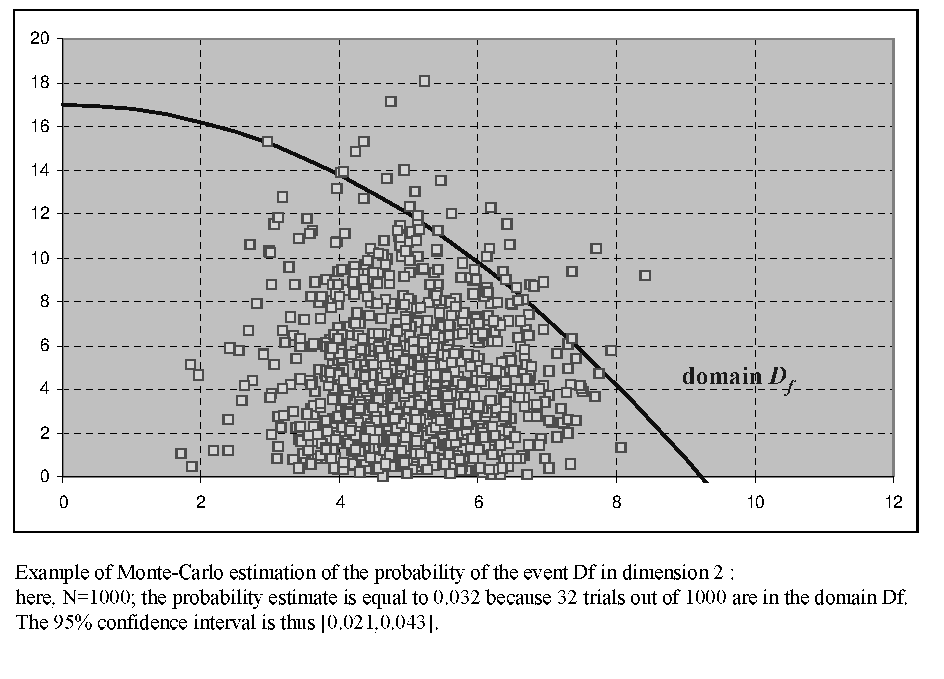
\includegraphics[scale=0.8]{Figures/MC2.pdf}
  \end{center}
}
{
  Direct sampling, Crude Monte Carlo method, Classical Monte Carlo integration
}

\Methodology{
  This method is used in step C and enables the probability of exceeding the threshold of an output variable (we refer to the probability of exceeding the threshold (critical region) because the inequality $g(\vect{X},\vect{d}) \leq 0$ by convention defines a reliability/critical region, and is in the general case the rewritten inequality of type $Z \geq \textrm{threshold}$ where $Z$ is a a random variable function of $\vect{X}$ and $\vect{d}$).

  This amounts to calculating the cumulative distribution function of the output variable at a point and thus propagating the uncertainty defined in step B using the model defined in step A.\\

  Input data:
  \begin{itemize}
  \item $\vect{X}$: random vector modelling the unknown variables defined in step A and for which the joint probability density function has been defined in step B,
  \item $\vect{d}$: vector of deterministic calculation parameters,
  \item $g(\vect{X},\vect{d}) \leq 0$: probabilistic criterion specified in step A,
  \end{itemize}

  Parameters:
  \begin{itemize}
  \item $N$: number of simulations to be carried out (samples to be taken) (maximal in the case where $\left( \textrm{CV}_{\widehat{P}_f} \right)_{\max}$ is specified, see next parameter),
  \item $\left( \textrm{CV}_{\widehat{P}_f} \right)_{\max}$: maximal coefficient of variation of the probability estimator (optional),
  \item $\alpha$: confidence level required for the confidence interval.
  \end{itemize}

  Outputs:
  \begin{itemize}
  \item $\widehat{P}_f$: estimation of the probability of exceeding the threshold (critical value/region),
  \item $\textrm{Var}({\widehat{P}_f})$: estimation of the variance of the probability estimator,
  \item $\widehat{P}_{f,\sup}-\widehat{P}_{f,\inf}$: length of the confidence interval.
  \end{itemize}
}
{
  The standard Monte-Carlo method requires very few special properties for the function $g$: it should be measurable and integrable but can be irregular, non-convex\ldots On the other hand, this method is not suitable when the probability to be estimated is small and when the CPU time needed to evaluate the criterion $g(\vect{X},\vect{d}) \leq 0$ is considerable. In practice, the standard Monte-Carlo method is not recommended except if one has (for $P_f < 10^{-2}$):
  \begin{align*}
    \frac{ \displaystyle t_\textrm{CPU} \left\{ g(\vect{X},\vect{d}) \leq 0 \right\} }{ \displaystyle P_f \times (\textrm{estimation precision})^2 } \leq \textrm{available machine time}
  \end{align*}
  where:
  \begin{itemize}
  \item $t_\textrm{CPU} \left\{ g(\vect{X},\vect{d}) \leq 0 \right\}$: CPU time needed to evaluation the criterion $\left\{ g(\vect{X},\vect{d}) \leq 0 \right\}$ for given data values of $\vect{X}$ and $\vect{d}$,
  \item estimation precision: desired limit for the coefficient of variation of the estimator,
  \item available machine time: desired limit on the total duration of the estimation.
  \end{itemize}

  Readers interested in the problem of estimating the probability of exceeding a threshold are referred to \otref{docref_C311_Form}{FORM}, \otref{docref_C311_Sorm}{SORM}, \otref{docref_C322_LHS}{LHS}, \otref{docref_C322_TI}{Importance Sampling} and \otref{docref_C322_DirectionalSimulation}{Directional Simulation}.

  The following provide an interesting bibliographical starting point to further study of this method:
  \begin{itemize}
  \item Robert C.P., Casella G. (2004). Monte-Carlo Statistical Methods, Springer, ISBN 0-387-21239-6, 2nd ed.
  \item Rubinstein R.Y. (1981). Simulation and The Monte-Carlo methods, John Wiley \& Sons
  \end{itemize}
}
